\documentclass[fleqn]{article}
\usepackage{amsmath}
\usepackage[dvips]{graphicx}
\bibliographystyle{plain}
\begin{document}

\section*{\center 1m diameter methane pool fire}
\subsection*{\underline{Problem Description}}
1m methane pool fire has become a valuable case for code validation, due to data
collected by~\cite{tieszen}.  At time $t=0$ the computational domain is set up to have 1m diameter methane inlet at the bottom wall. The rest of the boundaries are set up to simulate open boundaries. As simulation time progresses,
methane pool fire ignites and burns, exhibiting puffing behavior. This problem tests the ability of the Arches algorithm to handle non-adiabatic reacting flow.
 
\subsection*{\underline{Simulation Specifics}}
\begin{description} 
\item [Component used:] \hfill ARCHES
\item [Input file name:] \hfill methane\_1m.ups
\item [Command used to run input file:]\hfill mpirun -np 64 sus methane\_1m.ups
\item [Postprocessing command:]\hfill scirun methane\_1m.srn

\item [Simulation Domain:]\hfill    3 x 3 x 3 m
\item [Cell Spacing:]\hfill \\ 
3 x 3 x 3 cm (Level 0)

\item [Example Runtimes:] \hfill \\
 8 hours   (64 processors, 2.4 GHz Xeon (inferno cluster))

\item [Physical time simulated:] \hfill 0.428 sec.

\end{description}

\section*{\underline{Results}}
Figure~\ref{results1} shows a 2D center-plane contour plot of temperature at 
$t=0.428$ seconds. Code speed for methane simulation is relatively slow, but
the example cases for this release are limited to 8 hour 64 processors run time. So, figure~\ref{results1} is just a representation of what can be expected
after a run of this duration, much longer run times are required to gather statistics for experimental data comparison. As an example, figure~\ref{results2}
shows first puff leaving the simulation domain at $t=0.96$ seconds after
$26.5$ hours run time.
\begin{figure}
\includegraphics[scale=.85]{figures/methane_1m_420.ps}
\caption{2D center-plane contour plot of temperature at $t=0.428$ seconds.}
\label{results1}
\end{figure}
\begin{figure}
\includegraphics[scale=.85]{figures/methane_1m_960.ps}
\caption{2D center-plane contour plot of temperature at $t=0.96$ seconds.}
\label{results2}
\end{figure}
\newpage

\bibliography{../references}

\end{document}
